\documentclass{article}
\usepackage{icmc, amsmath}
\usepackage{graphicx}
\usepackage{url}                      % (handy if you reference a URL.)
\makeatletter
\def\url@leostyle{
  \@ifundefined{selectfont}{\def\UrlFont{\sf}}{\def\UrlFont{\small\ttfamily}}}
\makeatother
\urlstyle{leo}

%% These screw up HTML

\newcommand\T{\rule{0pt}{2.6ex}}
\newcommand\TT{\rule{0pt}{3.6ex}}
\newcommand\B{\rule[-1.2ex]{0pt}{0pt}}
\newcommand\BB{\rule[-2.2ex]{0pt}{0pt}}

\title{libIntegra: a system for software-independent multimedia module description and storage}

\twoauthors
{Jamie Bullock} {UCE Birmingham Conservatoire \\ Music Technology}
{Henrik Frisk} {Lund University\\ Malm\"{o} Academy of Music\\ Composition and Performance}

\begin{document}

\maketitle

\begin{abstract}
In this paper we describe a means of storing information about audio and message processing modules, which is not software specific. This information includes a module description, module instance data, and module implementation data. A novel XML file format and database schema are proposed, and we show how a newly developed library (libIntegra) can be used as a link between persistent storage on a networked server, and an existing software environment for audio. The library provides methods for instantiating and connecting modules in a given piece of software, and addressing them using Open Sound Control (OSC) messaging. An example scenario is discussed whereby the process of module data retrieval, de-serialization, instantiation and connection is managed from a remote GUI.
\end{abstract}

\section{Introduction}\label{sec:introduction}

libIntegra is part of the Integra project, a 3-year project led by UCE Birmingham Conservatoire in the UK and part financed by Culture 2000\footnote{\url{http://www.integralive.org}}. One aspect of Integra is to develop a new software environment to facilitate composing and performing in the context of interactive and live electronic music. In general, the project attempts to address the problems of persistent storage, portability and standardized intercommunication between different software (and hardware) systems for electronic music. It is a priority that all data relating to supported musical works, including scores, electronic parts, information about different versions and renderings of these works, biographical data, etc., should be stored on a web-accessible database, and that this data should be transferable to a variety of usable target applications.

Integra started as a way of standardising the construction of modules, and providing a generalised OSC namespace within the Max/MSP environment. As such it has similarity with the Jamoma\cite{Place:06}\footnote{\url{http://www.jamoma.org/}} and Jade projects\footnote{\url{http://www.electrotap.com/jade}}. However, it now differs substantially from either of these in that it has a strong emphasis on software independence, and persistent storage. Two other projects that aim to tackle problems that are similar to those which Integra attempts to address are Faust \cite{Orlarey:04}\cite{Orlarey:02}\footnote{\url{http://faust.grame.fr}} and NASPRO\footnote{\url{http://sourceforge.net/projects/naspro/}}. Furthermore, Integra is closely related to documentation and migration initiatives such as the PD Repertory Project\cite{Puckette:01}, Mustica\cite{Bachimont:03}, and the CASPAR Project\footnote{\url{http://www.casparpreserves.eu/}}, though the scope of the latter is much wider than that of Integra.

The Integra library is being developed as a foundation for the software development aspect of the Integra project. Its purpose is to make it possible to retrieve data (in particular the electronic sound processing part of the piece in question - the Max/MSP or PD patch for example) from the Integra database, and seamlessly load it into the required pieces of software. It is also our mission that it should be possible to load the same 'Integra collection' file (see \ref{subsec:module_collections}) in, or redirect parts of it to, a variety of different targets. Once loaded into its given target(s) the module collection will be addressable using a common OSC address space. The library should also support the instantiation of a module collection across multiple target applications for audio and multimedia.

\section{Integra modules}\label{sec:modules}

The basis of the Integra library is the concept of the Integra module. Integra modules encapsulate a specific piece of message or signal processing functionality. A module could perform a simple task like a numeric addition, or a complex task like emulating a specific synthesiser. In this section, we will outline how Integra modules and module collections are constructed.

\subsection{Module construction}\label{subsec:module_construction}

The minimum requirement for an Integra module is that it must have an interface definition. In addition, it may also have an implementation and module instance data. Of these, only the implementation is software specific.

\subsubsection{Module definition}\label{subsubsec:module_definition}

An Integra module definition is data that defines what attributes a module has, and what the characteristics of those attributes are. An Integra attribute is a symbolic name with which a value can be associated. The module definition doesn't store the actual values of attributes, instead it stores data about the attributes such as their names, descriptions, supported data types, maxima and minima, and default values. Typical module definition data is shown in Table \ref{tab:module_definition}.

\begin{table}
\begin{center}
\begin{tabular}{|l|l|}
\hline
\textbf{Field} & \textbf{Value} \\
\hline
Name  & Oscillator \\
\hline
Parent  & Module \\
\hline
Attributes & freq, phase \\
\hline
Attribute Unit Codes & 1, 2 \\
\hline
Attribute Minima & 0, 0 \\
\hline
Attribute Maxima & inf, 6.2831853071795862 \\
\hline
Attribute Defaults & 440, 0 \\
\hline
\end{tabular} 
\end{center}
\caption{Integra Oscillator interface definition}
\label{tab:module_definition}
\end{table}

The parent field is used to show an inheritance relation. All Integra module definitions could be thought of as class definitions, the members of which are all abstract (lack implementation), or interface definitions. The interface of a given class can inherit the interface of any other class, and supplement this with additional members. This definition hierarchy is the basis of the Integra database (see section \ref{sec:database}). 

\subsubsection{Module namespace}\label{subsubsec:module_namespace}

A module's namespace is derived from its definition. The namespace enables the values of attributes to be set, and module methods to be called  by using a symbolic naming scheme.  From the user's perspective, this will usually manifest itself as an OSC address space. The OSC address space for a sinus module is shown in table \ref{tab:module_namespace}. The sinus class inherits the oscillator class interface, which in turn inherits the module class interface, so all of these must be reflected in the module's namespace, and in turn must be represented in the implementation.

\begin{table}
\begin{center}
\begin{tabular}{|p{13em}|p{8em}|}
\hline
\textbf{OSC address} & \textbf{Purpose} \\
\hline
\begin{minipage}[0pt]{10em}
\small {
\begin{verbatim}/oscillator/freq <value>\end{verbatim}}\end{minipage}  & \small{Set the value of the 'freq' attribute} \\
\hline
\begin{minipage}[0pt]{10em}
\small{
\begin{verbatim}/oscillator/phase <value>\end{verbatim}}\end{minipage}  & \small{Set the value of the 'phase' attribute} \\
\hline
\begin{minipage}[0pt]{10em}
\small{
\begin{verbatim}/module/active <value>
\end{verbatim}} \end{minipage} & \small{Set whether or not the module is active} \\
\hline
\end{tabular} 
\end{center}
\caption{Integra Sinus module namespace}
\label{tab:module_namespace}
\end{table}

\subsubsection{Module implementation}\label{subsubsec:module_implementation}

The module implementation is the only software-specific data stored by Integra. It consists of a fragment of computer code, in one or more files, which when run or loaded by a particular piece of software will perform a specific audio or message processing task. In order that module implementations can be used by libIntegra, an implementation protocol must be devised for each software target. Integra currently provides implementation protocols for Max/MSP and Pure Data along with a growing selection of example module implementations and implementation templates. In practice, the implementation files are Max and PD 'abstractions' that provide a number of compulsory methods, and conform to the implementation protocol. A typical module implementation is shown in Figure {\ref{fig:sinus}}. 

\begin{figure}
\centerline{\framebox{
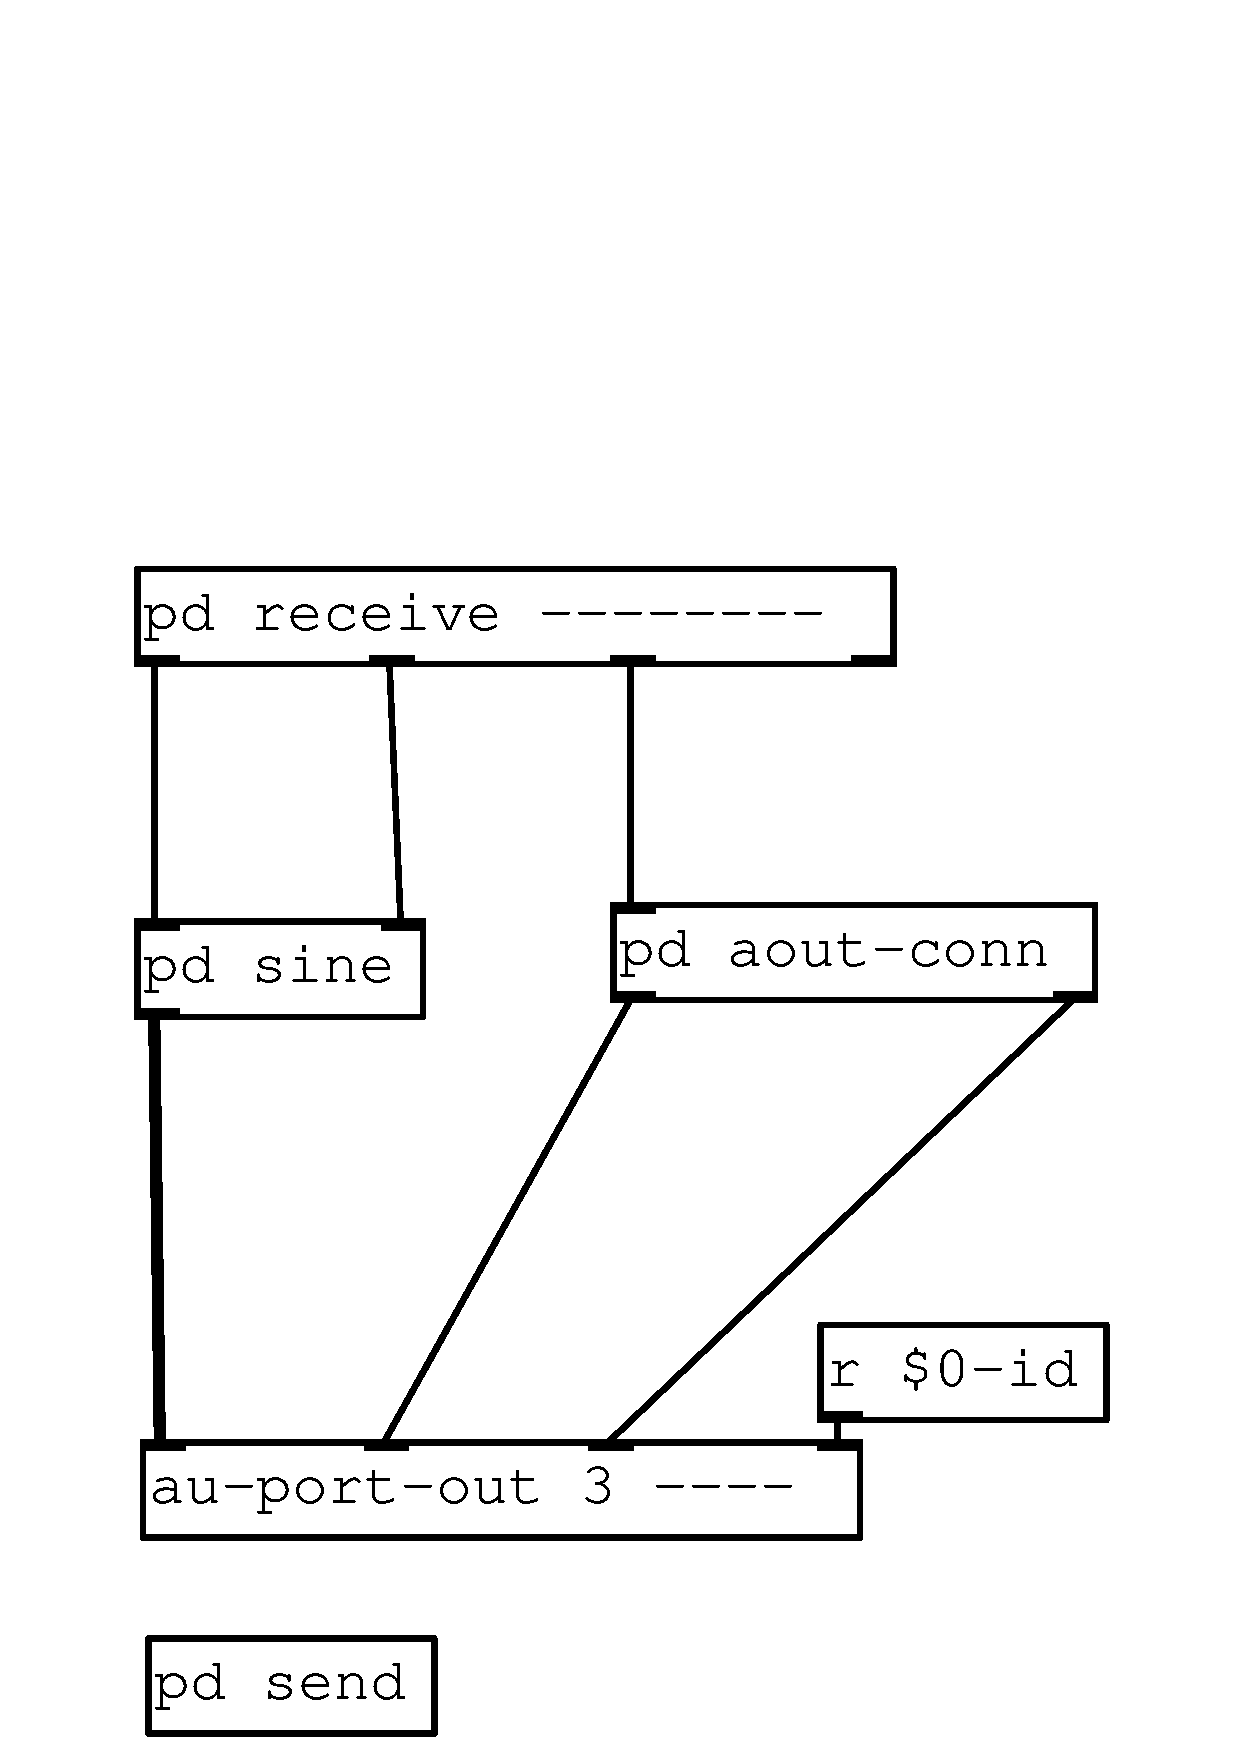
\includegraphics[width=14em]{img/integra-sinus}}}
\caption{An Integra sine wave oscillator implemented in PD}
\label{fig:sinus}
\end{figure}

A SuperCollider class to perform the same task, might look as follows:

{\small
\begin{verbatim}
Sinus : Oscillator {
    init{
     var freq, outPorts, server;
     freq = 440;
     outPorts = [1];
     actions = actions.add(
       {|val| this.server.sendMsg(
         ``/n_set'', nodeid, \freq, val)});
     nodeid = Synth(\Sinus, 
       [\freq, freq, \outport0, outPorts[0]]
       ).nodeID;
     super.init;
    }
}
\end{verbatim}
}

This implementation is very different from the PD sinus, not only because it is implemented in a different module host (i.e. SuperCollider), but also because it employs inheritance to provide much of its functionality. In SuperCollider we can use inheritance at the level of implementation to mirror the interface inheritance used in the Integra database, and conceptually between abstract Integra classes. The PD sinus must implement all of the interfaces inherited by the sinus class and its parents, right to the top of the class tree. The SuperCollider sinus only needs to implement the interface that is unique to it, implementations of inherited interfaces are inherited from the parent class: Oscillator. 

An eventual aim of Integra is to provide a protocol for constructing module implementations in a range of different software, and to develop a LADSPA/DSSI host that wraps plugins in an Integra-compliant manner.

\subsubsection{Module instance data}\label{subsubsec:module_instance_data}

Module instance data consists of the run-time state of all of its variable parameters. This data is stored in memory by the Integra library whilst a module is in use, and can be written to an XML file on demand. This data is stored in the Integra database in the module's instance table. However only one saved state can be associated with each module instance. If the user wishes to record state changes over time, then a separate 'Player' module must be used to store this data.

\subsection{Module collections}\label{subsec:module_collections}

An Integra collection consists of one or more Integra module instances. A collection can also contain other collections. These contained collections encapsulate the functionality of a number of connected Integra modules into a single entity and can be addressed and connected as if they were normal module instances. The facility is provided for collections to optionally expose the input and output parameters of the modules they contain. For example, the collection 'mySinus' might contain a Sinus module, which has the attributes Frequency and Phase, but the collection might only expose the Frequency attribute to the containing collection, whilst setting the Phase to some arbitrary constant value.

\subsection{Module ports}\label{subsec:module_ports}

Modules and collections are connected up to each other using Integra ports. Each port corresponds to an audio or messaging address, which has both a symbolic name and a numeric identifier (port ID). Port symbolic names correspond to a module's attribute names (e.g. 'freq'), and port numbers are derived implicitly from the index of the port in the module's attribute list. In addition to its port number, each module has a globally unique symbolic name (e.g. 'sinus1'), and an implicitly determined, globally unique numeric identifier (UID). The Integra library can be used to address any module port using either their fully-qualified symbolic name (e.g. '/sinus1/oscillator/freq'), or using a combination of their UID and port ID. It is an important part of the Integra module construction protocol that port ordering is always consistent. Otherwise a module implementation's port numbering will not correspond to the numbering expected by the Integra library.

From the perspective of the Integra library, database, and XML schema,
there is no distinction between audio and control rate ports. This
distinction is only made in the implementation. There is also no
conceptual distinction between input ports and output ports, a port is
just an address that can receive data and connect to other addresses.
This is illustrated in figure \ref{fig:sinus} where the first 'route'
object corresponds to ports one to four, which in turn correspond to
oscillator frequency, oscillator phase, the module 'active' setting, and
the audio output. In this example, ports one to three will set the
attributes of the sine oscillator when sent a numeric value, and report
their current value to any connected ports when sent an empty message.

\subsection{Connections}\label{subsec:connections}

For each module or collection, the Integra library stores a list of ports that each output port of a given module is connected to. One-to-many, many-to-one or many-to-many connections can easily be established. However, it is important to note that providing this functionality makes it a requirement for the software hosting the modules to support these routings. 

\begin{table*}
\begin{center}
\begin{tabular}{|p{25em}|p{21.5em}|}
\hline
\textbf{Command} \T \B & \textbf{Purpose} \\
\hline
\begin{minipage}[0pt]{20em}
\small {
\begin{verbatim}/load <module-name>\end{verbatim}} \end{minipage} \T & \small{Instantiate a module in a given target} \\
\hline
\begin{minipage}[0pt]{20em}
  \small {
\begin{verbatim}
/remove <module id>
\end{verbatim} 
}
 \end{minipage} \T
& \small{Remove a module instance} \\
\hline
\begin{minipage}[0pt]{20em}
\small {
\begin{verbatim}
/connect<module id> <port number> 
     <module id> <port number> 
\end{verbatim} 
}
 \end{minipage} \TT
& \small{Connect two ports} \BB \\
\hline
\begin{minipage}[0pt]{20em}
\small {
\begin{verbatim}
/disconnect <module id> <port number> 
         <module id> <port number> 
\end{verbatim}
}
 \end{minipage} \TT
& \small{Disconnect two ports} \BB \\
\hline
\begin{minipage}[0pt]{20em}
\small {
\begin{verbatim}/send <module id> <port number> <value> 
\end{verbatim} 
}
 \end{minipage} \T
& \small{Send a value to a port} \\
\hline
\begin{minipage}[0pt]{20em}
\small {
\begin{verbatim}
/direct <module id> <state> \end{verbatim}
} \end{minipage} \T
& \small{Toggle direct message passing for a module instance} \BB \\ 
\hline
\end{tabular} 
\end{center}
\caption{Instance host OSC scheme}
\label{tab:lib_namespace}
\end{table*}

\section{IXD (Integra eXtensible Data)}\label{sec:ixd}

In order to store modules, module collections, and performance data in a software-neutral manner, a bespoke Integra file format was developed. XML was chosen as the basis for this since it is relatively human-readable, can be transformed for a variety of output targets, and has a number of excellent tools for parsing, reading and writing. The library currently uses the libxml2\footnote{\url{http://xmlsoft.org/}} library to provide much of its XML processing functionality.

Rather than keeping all data needed to store an Integra collection in a single file we make use of the XML Linking language (XLink\footnote{\url{http://www.w3.org/TR/xlink/}}) to link in relevant resources. This makes for more efficient parsing and helps to keep file sizes small.

\subsection{Integra module definition}\label{subsect:integra_class_definition}

Perhaps the most important part of the IXD specification is the module definition file. It is the XML representation of an Integra module (see \ref{subsubsec:module_definition}). These files are created and updated through the database interface and stored locally for offline access in a gzipped archive. Each file contains the class and module definitions of one unique module and a link to the parent class from which it inherits properties:

{\small
\begin{verbatim}
<Class>
 <ClassDefinition>
   <className>Sinus</className>
   <classParent ...
        xlink:href="Oscillator.xml">
        Oscillator
   </classParent>
    ...
 </ClassDefinition>
 <ModuleDefinition>
    ...
 </ModuleDefinition>
</Class
\end{verbatim}
}
All documents that are part of the Integra documentation system must have a class definition - it represents the super class of the Integra class hierarchy and it defines those attributes shared by all kinds of data - performance data, biographical data, etc. (see section \ref{subsubsec:module_definition}). The module definition is specific to the notion of \emph{modules} as defined in section \ref{sec:modules}.

A part of the body of the module definition IXD file containing the definition shown in Table \ref{tab:module_definition}, would contain the following construct (please note that only the \emph{freq}-attribute is included):

{\small
\begin{verbatim}
<attributeUnitCodes> 
  <index id="0">
    <name>Hz</name>
    <description>
        The value in Hz (0 - INF).
    </description>
  </index>
</attributeUnitCodes>
<attributeMinima> 
  <index id="0">
     <value>0</value>
  </index>
</attributeMinima>
<attributeMaxima> 
  <index id="0">
    <value>INF</value>
  </index>
</attributeMaxima>
<attributeDefaults>
   <index id="0">
     <value>440</value>
   </index>
</attributeDefaults>
...
\end{verbatim}
}

Each module and each of its attributes may also hold a documentation reference. This allows the implementing host for this module to make a call to the instance host to bring up on-line documentation, for this attribute or for the module itself. The link points to a file included in the local archive of module descriptions.

{\small
\begin{verbatim}
<classAttributesDocumentationIDs>
  <index id="0"
         ...
     xlink:href="FrequencyDoc.xml">
  </index>
</classAttributesDocumentationIDs>
\end{verbatim}
}

\subsection{Integra collection definition}\label{subsect:integra_collection_definition}

Once a module is defined and stored in an IXD file it may be instantiated. Instances of classes of modules along with their inter-connections are stored in a collection file which is the Integra equivalent of a PD or Max/MSP 'patch'.

In a collection file each module instance is represented by a locator that points to the definition of the class to which the instance belongs. Connections between ports are represented by \emph{arcs} between resources (pointing to definitions of individual addresses) in the module definition file pointed to by the locator. Finally, it also holds references to performance data files.

\subsection{Integra performance and preset data}\label{subsect:integra_preset_data}

The performance and preset data files store information about the current and previous \emph{N} states of the instance stored at a specified time resolution, stored presets, and sequences of dynamic data. As was mentioned in section \ref{subsubsec:module_instance_data}, this information is only available to instances, or a group of instances, which holds a reference to a special kind of data module, i.e. this file represents an instance of this data module which in turn is associated with a specific module instance or group of module instances.

% \subsection{The IXD file format - summary}
\subsection{Serialization layer}\label{sec:serialization_layer}

To facilitate the conversion between flat XML files conforming to the IXD specification, and a memory-resident representation of the data, a serialization library component has been developed (see \ref{subsec:serialization}). The serialization layer is the link  between the database and the local file system (see figure \ref{fig:model}).

The serialization component provides functions for loading, saving and modifying XML, and is used by the instance host (see \ref{subsec:instance_host}), the database (see \ref{sec:database}) and/or any other application interfacing with the library. For example, on the database server, the serialization layer is made available to the python-based web interface via a SWIG-generated interface.

The IXD format is specified and documented in several XML Schemas\footnote{\url{http://www.w3.org/XML/Schema}}. The XML Schema for the module definition files is closely correlated to the database schema and they share the same versioning system. Any file conforming to the file format can be validated against a specific schema version and conditional actions may be performed on them as appropriate.

Finally, we are also working on an Integra specific XSL Transformation\footnote{\url{http://www.w3.org/TR/xslt}} specification for automatic generation of XHTML and/or PDF documentation of a given module or collection of modules. In practice this means that once the user has created his or her own Integra collection for a piece or a project, and uploaded it to the database a documentation file for this collection is automatically created.

\section{Database}\label{sec:database}

For persistent storage of module data and other data relating to musical works we have designed and configured an on-line database. The database comprises a postgresql back-end, and a web-based UI written in Python. Postgres was chosen because of its reliability, maturity and close-coupling with the data-structures to be stored. Because postgres is an object-relational database management system (ORDMS), we were able to utilise the facility to create inheritance relations between tables, mirroring inheritance between module classes. We also make extensive use of postgres' array type.

In the Integra database, the module definitions are stored in one table, with references to data in a number of supplementary look-up tables. For example, the module definition shown in Table \ref{tab:module_definition} would be stored in a single row in the Module Definitions table. Data in fields such as 'Attribute Unit Codes' are stored as integers that are used as indices to a look-up table. This is done to ensure data consistency, efficiency of storage and fast look-up.

The 'Attribute Units' look-up table might look as shown in table \ref{tab:lookup_table}.

\begin{table} 
\begin{center}
\begin{tabular}{|l|l|}
\hline
\textbf{Field} \T \B & \textbf{Value} \\
\hline
1 & Hertz \T \\
\hline
2 & Radians \T \\
\hline
\end{tabular} 
\end{center}
\caption{Typical look-up table}
\label{tab:lookup_table}
\end{table}

\subsection{Database UI}\label{subsec:db_ui}
The only way in which users may add new, or edit existing module definitions is via a web-based interface. It also provides mechanisms for uploading and downloading module definitions, and collections.
Once a module definition has been added to the definitions table, the database schema is extended through the addition of a corresponding table to hold the new module's instance data. When a module definition is added to the database, the module's parent is specified, and only attributes that differ from those provided by its parent are added. An inheritance relation is then created between the new module's instance table, and the parent module's instance table. This means that all of the parent module's attributes then become available to instances of the child module.


\section{(Integra)tion via the library}\label{subsec:db_lib}

libIntegra is a cross-platform shared library, mostly written in ISO C89 compliant C, and packaged using the GNU autotools tool chain. It consists of a common API, and a number of optional components.

\subsection{Serialization component}\label{subsec:serialization}

As mentioned in \ref{sec:serialization_layer} the database also makes use of the serialization component. When the user requests a particular module collection, the database is queried for the relevant data, and the serialization library component is used to generate a number of XML files. These files are in turn bundled into a gzipped archive and stored locally. The program linked to the Integra library can then use the same XML handling functions to de-serialize the data, and form an in-memory representation of it.

\subsection{Instance host}\label{subsec:instance_host}

As well as a serialization component the library provides an instance host, which is responsible for keeping a record of each module's run-time state. This includes the values that any of its ports have, and any connections that are made between modules. The instance host acts as an OSC server (using the liblo library\footnote{\url{http://liblo.sourceforge.net/}}), and operations can be performed on modules by sending OSC messages to it. The instance host supports a simple efficient syntax as shown in table \ref{tab:lib_namespace}.

Module instances can either communicate with each other through the instance host using OSC, or directly using an environment-specific messaging system. The method to be used is determined by the value of the module's 'direct' flag. If messages pass through the Instance host, it means that various operations can be performed on the data as it passes through. This includes:
\begin{itemize}
\item Type checking
\item Range checking
\item Unit conversion
\item Type conversion
\end{itemize}

All of these can be validated against the module definition held in memory.
 
\subsection{Library/target bridge}\label{subsec:bridge}

In order to instantiate modules in a target environment, and send data to these modules in an efficient way, the Integra instance host needs a way to communicate directly with the environment. This is done using a target-specific bridge, which is a dynamically loaded binary shared object hosted 'inside' the instance host. The library provides a very simple API, that each target-specific bridge must conform to. The instance host has no knowledge of the software being used to host the module instances so the bridge acts like a translator receiving function calls, and performing the relevant target-specific actions. These actions include instantiating modules, removing them and connecting them. Most OSC commands supported by the Instance host have a corresponding function in the bridge.

It is the plug's software-specific communication mechanism that determines the protocol used to construct module implementations. It is possible, although not necessarily desirable to have several bridgess for a given target, each of which elicits a different approach to module construction. This might be useful for compatibility with existing modularisation efforts, such as the Jamoma project, or PD Faust modules.

\begin{figure*}
\centerline{\framebox{
\includegraphics[width=45em]{img/library_model}}}
\caption{A model of the parts constituting libIntegra and how the library interfaces with other parts of the system.}
\label{fig:model}
\end{figure*}

\subsection{Module host}\label{subsec:module_host}

The module host is not part of libIntegra, it is any software that hosts Integra modules. Typically, a module host will be dynamically linked to libIntegra at compile time. At run time the module host can make direct calls to functions in the instance host and also make use of the Instance host OSC interface. Typically the OSC interface is used for communication from the individual modules.  Communication from the Instance host to the module host and modules is always achieved through the bridge.

It is also possible for the module host to be a standalone application that doesn't link to libIntegra. In this case the bridge will usually use a network-based protocol such as OSC to communicate with the module host. A Unix pipe or socket is another possibility for this type of setup.

\subsection{Inter-library communication}\label{subsec:interlib}

An arbitrary number of libIntegra instances may be running on the same computer or on any number of networked computers. Each libIntegra instance can be running in a new instance of a common module host, or a completely different module host. A typical configuration is shown in Figure \ref{fig:model}. 

When multiple libIntegra instances are used, only one (the master), can make use of the serialization layer to load and save Integra module instance data and collections. This is to prevent several versions of the same collection being opened by different library instances, and becoming unsynchronised. If the user or developer knows that the serialization layer will not be required, the library can be compiled without it.

The Instance host contains mechanisms for inter-library communication and auto-discovery. This is mostly achieved through OSC messaging, and facilitates the loading of Integra collections across several module hosts, with transparent state saving.

\subsection{libIntegra package}\label{subsec:cli}

In addition to providing the instance host and serialization components, which constitute the bulk of the libIntegra binary shared object, the libIntegra package also provides a number of other useful tools. These include a CLI (command line interface) through which all operations can be performed in a non-GUI mode, a number of example bridge implementations, and a number of example module host implementations.

\section{Use case scenario}\label{sec:use_case}

We will now describe a typical use case for the Integra library involving the on-line database, and a DSP environment running locally. The data flow is summarized in figure \ref{fig:model}. We will assume that the database is empty.

Firstly, 'user A' (\emph{A} hereafter) will create a couple of module implementations following the Integra module creation protocol. Once this is done, \emph{A} will enter the modules' definitions into the database using the on-line web interface, and upload the implementations using an on-line form. 

'User B' (\emph{B} hereafter) will then launch the required GUI and DSP engine (these may be provided by the same program), both of which provide linkage to libIntegra. The GUI will call the serialization component for an up-to-date version of the available modules and their definitions which in turn acquires an archive of the definitions and the module implementation files.

Now that the GUI is aware of the available module definitions, modules can be instantiated and inter-connected in the Engine. If these are graphical modules, they will be instantiated in the GUI. In this example, \emph{B} creates a slider in the GUI, and a sinus oscillator in the engine, and connects the port corresponding to the 'position' attribute of the slider to the port corresponding to the 'frequency' attribute of the sinus oscillator.

The user can modify the state of these modules by moving the slider. Once \emph{B} is satisfied with the connected modules, the connection graph, and the current module state, it can be saved back to the Integra archive as XML, again by calling functions in the Integra library via the GUI. If the user has an Internet connection, then the new module collection can be written directly to the database using XML-RPC.

Any new user can now download the newly created module collection, load and modify it, and then commit their changes back to the database. The database employs a versioning system, so that at any point a collection can be reverted to a previous save-state.

\section{Project status}\label{sec:status}

The Integra library is currently hosted on sourceforge.net. We have a small but active developer community, which is growing slowly as the project progresses. It is important to note that the Integra library is only one element of the Integra environment. The Integra environment is the core goal of the development strand of the Integra project, and seeks to provide a complete solution for composers and performers working in music with Interactive live electronics. The library provides the foundation for this environment, but we are also developing a bespoke GUI for composers and performers to work with.

The library and the GUI are both currently in pre-alpha development.

\subsection{Future work}\label{subsec:future}

One of current priorities is to populate the Integra database with a large number of module definitions and implementations. However, we would like to keep the amount of implementation-specific data we store to an absolute minimum. The first step in this has been to separate out the module definition, namespace (derived from the definition), instance data, and implementation. We would now like to explore ways of storing the data encoded by the implementation in an software-neutral manner. One way to do this might be to create a set of implementation primitives, and then create more complex modules from these using Integra collections as an encapsulation mechanism. Another possibility would be to create a simple Integra scripting language that could be used in addition to module encapsulation, or alongside a DSP description language such as Faust. 

\section{Conclusion}\label{sec:conclusion}

We have outlined a robust, cross-platform, software-independent means of storing and loading module data. In addition we have discussed the facilities that the Integra library provides for loading, saving, instantiating and managing modules and collections of modules. The next stage in our work will entail a phase of alpha and beta testing, both internally and with our end users. The aim of the Integra project is to improve the usability of software for working with live electronics, and to provide a mechanism for the sustainability of the musical works it is used to create. libIntegra should ultimately provide a foundation for this.

\begin{thebibliography}{citations}

\bibitem{Orlarey:04} Orlarey, Y. and Fober, D. and Letz, S.
''Syntactical and semantical aspects of FaustSoft Computing''
{\it Soft Computing - A Fusion of Foundations, Methodologies and Applications}, vol. 8, no. 9, 2004

\bibitem{Orlarey:02} Orlarey, Y. and Fober, D. and Letz, S.
''An Algebra for Block Diagram Languages''
{\it Proceedings of the International Computer Music Conference}, ICMA, USA, 2002.

\bibitem{Place:06} Place, T. and Lossius, T.
''Jamoma: A Modular Standard for Structuring Patches in Max''
{\it Proceedings of the International Computer Music Conference}, ICMA, USA, 2006.

\bibitem{Puckette:01} Puckette, M.
''New Public-Domain Realizations of Standard Pieces for Instruments and
Live Electronics''
{\it Proceedings of the International Computer Music Conference}, ICMA, USA, 2006.

\bibitem{Bachimont:03} Bachimont, B. and Blanchette, J.-F. and Gerzso, A. and Swetland, A. and Lescurieux, O. and Morizet-Mahoudeaux, P. and Donin, N. and Teasley, J.
''Preserving interactive digital music: a report on the MUSTICA research initiative''
{\it Web Delivering of Music, 2003.} 2003 WEDELMUSIC. Proceedings. Third International Conference on Web Delivering of Music.

\end{thebibliography}

\end{document}
